\documentclass[11pt, oneside]{article}
\usepackage[margin=1in]{geometry}
\geometry{letterpaper}
\usepackage{booktabs}
\usepackage{hyperref}
\usepackage{enumitem}
\usepackage{float}
\usepackage{caption}
\usepackage{subcaption}
\usepackage[numbers]{natbib}
\usepackage{graphicx}
\usepackage{amssymb}
\usepackage{amsmath}
\usepackage{array}
\usepackage{longtable}
\usepackage{xcolor}
\usepackage{tabularx}
\usepackage{setspace}
\hypersetup{
    colorlinks=true,
    linkcolor=blue,
    citecolor=blue,
    urlcolor=blue
}
\newcommand{\fillin}[1]{\textcolor{red}{[#1]}}
\captionsetup{font=small,skip=4pt}
% ============================================================
% TITLE BLOCK --- students must keep this format
% Filename of the compiled PDF must be:
% CS781-CP-[Firstname]-[Lastname]-[RollNo]-report.pdf
% ============================================================
\title{CS781 Capstone Project:\\
In-House Legal Intelligence System}
\author{
    Wren Oswin  \\
    261110073 \\
    wrenoswin26@iitk.ac.in\\
    Indian Institute of Technology Kanpur (IIT Kanpur)
}
\date{}
\begin{document}
\maketitle
\begin{abstract}
A law firm cannot send privileged documents to third-party language-model APIs, so I built a self-hosted legal NLP
stack on one 12\,GB laptop GPU. In Phase~1 I pretrained four Transformer families from scratch (decoder-only,
encoder-decoder, prefix-LM and a sliding-window efficient model); the best is a 140M-parameter LLaMA-style decoder
trained on 600M tokens of Acts, Supreme Court, High Court and Tribunal text mixed 35/35/15/15. Every later model
(legal NER, rhetorical roles, judgment prediction, statute identification, summarization and prior-case retrieval)
was initialised from these checkpoints and adapted with techniques I implemented from scratch, including LoRMA and
knowledge distillation. Four findings recur: the Phase-1 architecture ranking carries over to downstream tasks;
LoRMA, training under 3\% of the weights, matches or beats full fine-tuning of the same backbone; soft-label
distillation lets a 58M student match or beat its 140M teacher, whereas sequence-level distillation hurts; and the
size of the validation set decides which differences can be trusted.
\end{abstract}

% ============================================================
\section{Competition Result}
% ============================================================
\noindent
\textbf{Codabench username:} w\_261110073
\hfill
\textbf{Roll number:} 261110073
\medskip

\noindent
Table~\ref{tab:leaderboard} reports the best valid score of each phase. Code and documentation, with a README for
every phase and submission:\newline \url{https://github.com/WrenOswin/In-House-Legal-Intelligence-System}.
\begin{table}[H]
\centering
\caption{Official phase scores and ranks.}
\label{tab:leaderboard}
\begin{tabular}{clccc}
\toprule
Phase & Task & Primary metric (value) & Rank & Valid submissions \\
\midrule
1 & Legal LM Pretraining & BERTScore F1 0.8321 & 61 & 6 \\
2 & Legal NER & Strict macro-F1 0.5590 & 41 & 11 \\
3 & Rhetorical role prediction & Macro-F1 0.4950 & 66 & 22 \\
4 & Court judgment prediction & Macro-F1 0.7771 & 27 & 11 \\
5 & Legal statute identification & Macro-F1 0.4035 & 32 & 9 \\
6 & Abstractive summarization & BERTScore F1 0.8424 & 55 & 7 \\
7 & Prior Case Retrieval (PCR) & Micro-F1@7 0.4312 & 20 & 6 \\
\bottomrule
\end{tabular}
\end{table}
\noindent
\textbf{Total valid Codabench submissions across all phases:} 72
\quad
\textbf{Date ranks were recorded:} 07-11-2026
\medskip

% ============================================================
\section{Introduction and Problem Description}
% ============================================================
Privileged client material cannot leave a firm's infrastructure, which rules out commercial LLM APIs. The capstone
therefore asks for a compact legal language model trained from scratch, and evidence that it supports seven tasks
drawn from IL-TUR~\cite{joshi2024iltur}. Phase~1 continues a 512-word prompt with exactly 128 words (BERTScore
F1~\cite{zhang2020bertscore}). Phase~2 (L-NER) outputs \texttt{[start, end, label]} character spans for 12 entity
types under strict macro-F1, so a span off by one character is wrong. Phase~3 assigns one of 13 rhetorical roles to
every sentence of Corporate Law (CL) and IT judgments (macro-F1). Phase~4 predicts a binary outcome for
ILDC~\cite{malik2021ildc} cases (macro-F1). Phase~5 predicts the set of applicable statutes out of 100 (macro-F1).
Phase~6 writes an abstractive summary of a judgment (BERTScore F1). Phase~7 returns seven ranked candidates from each
query's pool (micro-F1@7).

The constraints shaped every design. The foundation had to have 50M--300M parameters and be trained from scratch;
Phases~2--7 could use no other pretrained weights or external data, had to use all four Phase-1 architectures, and
had to include three adaptation techniques (LoRMA compulsory) plus knowledge distillation. From Phase~3 the TAs
required every technique to be written from scratch, so my models, adaptation methods and training loops use only
\texttt{torch}, \texttt{numpy}, \texttt{regex}, \texttt{scipy} (sparse BM25), \texttt{psutil} and the standard
library; outside the models, \texttt{scikit-learn} fits the Phase-6 sentence-salience regression and
\texttt{rouge-score} computes local ROUGE. Everything ran on one Windows
laptop with an RTX~5070~Ti Laptop GPU (12\,GB), comparable to a free Colab/Kaggle GPU. I studied how architecture,
scale and data budget affect a compact legal LM; whether and how its representations transfer; whether a 58M student
can replace a 140M teacher; how to encode documents longer than the context; how decoding and thresholds affect the
metrics; and how far local validation can be trusted. Each phase was built end-to-end. I deliberately did not
attempt cross-encoder re-ranking, reinforcement-learning post-training, or pipelining one phase's predictions into
another; every task model is a separately fine-tuned descendant of the Phase-1 checkpoints.

% ============================================================
\section{Data Analysis and Preprocessing}
% ============================================================
\subsection{Sources and official splits}
I used only \texttt{Exploration-Lab/CS-781-Capstone} and its official configurations (Table~\ref{tab:data}).
Without a dev split (Phases~1, 2, 6) I held out training data: a slice of the Phase-1 mixture, a stratified
14-document NER split giving every label 17--23\% of its mentions, and 300 summarization documents. In Phase~4 the
released \texttt{test.json} carried labels and \texttt{dev.json} contained every test document with its label; I
dropped all labels on load, validated on the 994 dev documents outside the test set, and reported the leak. In
Phase~5 I removed exact duplicates from training and training duplicates from validation.

\begin{table}[t]
\centering\small
\caption{Splits and the statistics that drove design (tokens are my BPE tokens).}
\label{tab:data}
\setlength{\tabcolsep}{3.5pt}
\begin{tabular}{@{}llll@{}}
\toprule
Ph. & Train / val / test & Length & Labels \\
\midrule
1 & $>$4.5B tokens (600M used); 1{,}000 prompts & 512-word prompt & -- \\
2 & 56 / 14 docs (folds 1--2); 35 test & median 5.6k tokens & 12 types, 8{,}393 spans \\
3 & 80 / 10 / 10 docs (CL + IT) & 120--184 sentences/doc & 13 roles \\
4 & 31{,}652 / 994 / 1{,}517 docs & median 3.5k tokens & 41\% positive (val 50\%) \\
5 & 42{,}315 / 10{,}037 / 13{,}019 docs & median 550--700 tokens & 100 statutes, 3.7/doc \\
6 & 6{,}728 / 300 / 100 judgments & 3.1k-word doc, 640-word summ. & -- \\
7 & 827 / 118 / 237 queries & median 4.5k tokens & 4--5 relevant/query \\
\bottomrule
\end{tabular}
\end{table}

\subsection{Corpus statistics that actually informed design}
The Acts source holds only about 150M training tokens; the judgment sources supply the rest of the 4.5B. I weighted
Acts and Supreme Court at 35\% each and High Courts and Tribunals at 15\% each, favouring the cleanest registers, and
my data builder passes a source's unfilled share to the others. Prompt plus continuation is about 800 tokens, so a
1{,}024-token window suffices in Phase~1, but downstream documents are several times longer
(Table~\ref{tab:data}), which drove most later design. Figure~\ref{fig:data}(a) shows the NER imbalance
(\textsc{date} 1{,}575 vs.\ \textsc{r.counsel} 184 mentions). No gold spans overlap, but one string can carry several
labels (``Union of India'' is \textsc{resp} 28 times, \textsc{app} 14, \textsc{prec} 4, \textsc{auth} 4), and party
entities sit in the header (median relative position 0.15--0.27). In RR (Figure~\ref{fig:data}b), 93.7\% of CL and
75.4\% of IT sentences repeat the previous role, so copying the previous gold label already scores 0.754 on dev;
Issue, Dissent and PrecedentOverruled are extremely rare, the last two absent from dev.

\begin{figure}[t]
\centering
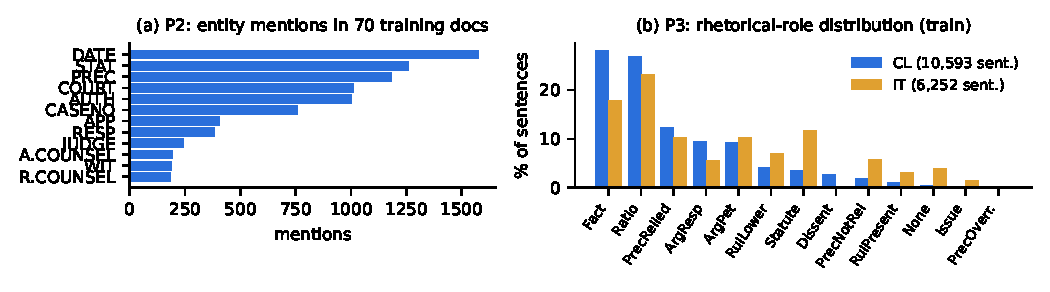
\includegraphics[width=\linewidth]{figures/fig_data.pdf}
\caption{(a) Entity-type frequencies in the Phase-2 training folds. (b) Rhetorical-role shares in CL and IT training data.}
\label{fig:data}
\end{figure}

CJPE validation and test documents are balanced, older (1950--90) and lower-cased, unlike the 41\%-positive, cased
training set. A TF-IDF probe showed the evidence is spread out (logistic regression 0.690 on the whole document, 0.640
on the last 512 words, 0.593 on the first 512). In LSI the rarest statute still has 272 training documents, the top 20
statutes carry 60\% of label mass, pairs co-occur strongly, and statute mentions are masked, so they must be inferred
from facts. In summarization about a third of reference bigrams are absent from the source, salience is flat after
the first 10\% of a judgment, and the first $\approx$1.3k tokens contain only 57\% of the reference's content words.
In PCR every query also sits in its own pool, gold sets range from 1 to 92 cases, and citations are masked; because
many queries have fewer or more than seven gold cases, a perfect ranker scores only 0.618 on dev.

\subsection{Preprocessing}
My BPE tokenizer~\cite{sennrich2016bpe} (32k and 35k vocabularies, trained on 100M characters) uses a Unicode-aware
pre-tokenizer that splits numbers into groups of at most three digits, keeping section numbers and years
compositional; five special tokens (e.g.\ \texttt{<|bos|>} and \texttt{<|sep|>}) frame downstream inputs. Dataset masks such as \texttt{<SECTION>} or \texttt{<CITATION>} would
cost 3--6 pieces, so each is mapped to one existing token. CJPE text is lower-cased and whitespace-normalised in every
split. For L-NER the text is never modified: the tokenizer returns each token's character span, gold spans become BIO
tags on those tokens, and predictions are mapped back through the same offsets. The original pre-tokenizer glued
entity-final punctuation to words (``SCC 47].''), leaving 152 gold ends inside a token, so the NER tokenizer splits
punctuation into single characters; a gold$\rightarrow$BIO$\rightarrow$span round trip then scores 0.9944. Documents are
processed in windows overlapping by half. RR uses the official sentence lists unchanged, packed into the backbone
window with newline separators (at most 128 tokens per sentence). Phases~4, 5 and~7 split documents into 512-token
chunks: up to four per document in training and 8 (CJPE, LSI) or 16 (PCR) evenly spaced chunks at inference. In PCR,
queries and candidates share one encoder and truncation policy; training chunks are chosen by trigram overlap with the
paired document. Summarization uses importance-based source selection (Section~\ref{sec:p6}).

% ============================================================
\section{Approach and Model Evolution}
% ============================================================
\subsection{Phase-1 foundation model}
All four architectures share LLaMA-style components~\cite{touvron2023llama} (pre-norm RMSNorm~\cite{zhang2019rmsnorm},
rotary positions~\cite{su2021roformer}, SwiGLU~\cite{shazeer2020glu}, no biases, tied embeddings), so differences come
from the overall design. \textbf{A} is a causal decoder-only stack. \textbf{B} encodes a 768-token prefix bidirectionally
and decodes a 256-token continuation with cross-attention. \textbf{C} is a prefix-LM with a bidirectional prefix,
causal continuation and segment embedding. \textbf{D} uses 256-token sliding-window attention~\cite{beltagy2020longformer}
with full attention every fourth layer, grouped-query attention~\cite{ainslie2023gqa} and a 2{,}048-token context. The
final model (Figure~\ref{fig:system}a) is A with 12 layers, 12 heads, $d=768$, SwiGLU hidden size 3{,}072, a
1{,}024-token context and a 35k vocabulary: 140.15M parameters, checked by a parameter count after construction.

\begin{figure}[t]
\centering
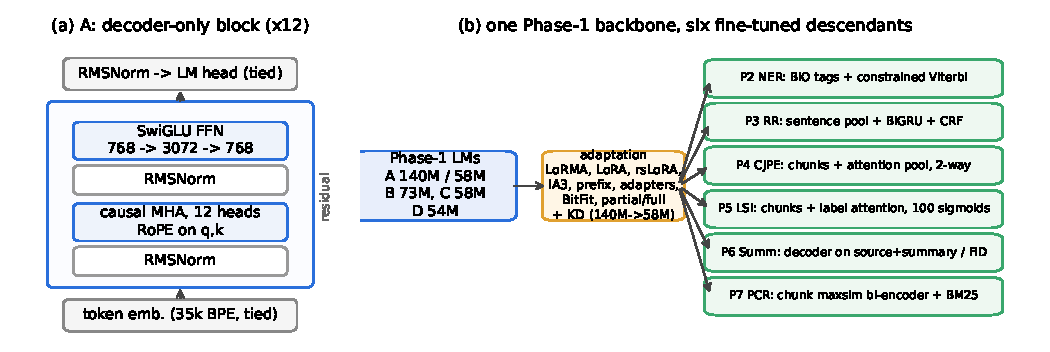
\includegraphics[width=\linewidth]{figures/fig_system.pdf}
\caption{(a) The final Phase-1 model. (b) The system: Phase-1 checkpoints, adapted with one of my techniques, feed six task heads.}
\label{fig:system}
\end{figure}

I first compared the four families at a fixed 200M-token budget and 54--73M parameters. A won on validation loss and
BERTScore (Table~\ref{tab:variants}), which I attribute to learning signal per token: A and D learn from every token,
C only from the continuation ($\approx$45\%), B from 256 of every 1{,}024 tokens read, and D's long context is useless
at 800 tokens. I then scaled A to $d$640 on 450M tokens and $d$768 on 600M tokens (434 minutes). A
MobileLLM-style~\cite{liu2024mobilellm} deep-thin variant (23 layers, $d$576, 9 query / 3 K/V heads) with a KV cache tied
the best model at 6\% fewer parameters (0.8314 vs.\ 0.8321) but trained 19\% slower; since it changed shape and
attention together, the effects cannot be separated. Submissions use temperature 0.8, top-$k$ 50, top-$p$ 0.95 and a
repetition penalty of 1.1 over 256 tokens, generating up to 512 tokens and truncating to 128 words; a first 320-token
budget left two outputs short when loops (``L.P.(C) L.P.(C)\,\ldots'') consumed it. The KV cache cut test generation
from about two hours to minutes, with token-identical fp32 outputs.

\subsection{Transfer protocol (Phases 2--7)}
Every task model starts from a Phase-1 checkpoint; only heads are new. Classification and retrieval use B's encoder
(42M). A~$d$768 is the main backbone, and the 58M A, B, C, D models give the other architectures and the KD students.
For summarization I re-implemented the forward passes and verified that they reproduce the original losses exactly.
I implemented ten techniques. Full and partial fine-tuning train all weights or the top four of eight blocks plus the
final norm. LoRA~\cite{hu2022lora} adds $\tfrac{\alpha}{r}BAx$ to a frozen $W_0x$ ($B=0$ at start), and
rsLoRA~\cite{kalajdzievski2023rslora} scales by $\alpha/\sqrt{r}$. LoRMA~\cite{bihany2025lorma} is multiplicative; since
$(BA)W_0$ alone has rank at most $r$, I use the identity-inflated form
\begin{equation}
h=\bigl(I+\tfrac{\alpha}{r}BA\bigr)W_0x = W_0x+\tfrac{\alpha}{r}B\bigl(A(W_0x)\bigr),
\end{equation}
evaluated right-to-left at $O(dr)$ cost per token, starting exactly at the pretrained model, on the attention and
SwiGLU projections. IA\textsuperscript{3}~\cite{liu2022ia3} rescales keys, values and FFN activations; prefix
tuning~\cite{li2021prefix} learns per-layer key/value prefixes through an MLP (inside D's blocked sliding-window
kernel); Houlsby~\cite{houlsby2019adapters} and Pfeiffer~\cite{pfeiffer2021adapterfusion} adapters add bottleneck MLPs;
and for BitFit~\cite{benzaken2022bitfit} I added zero-initialised biases to my bias-free backbones.

Distillation~\cite{hinton2015distilling} uses a fine-tuned 140M teacher and a 58M student with different tokenizers
(35k vs.\ 32k), so I distil at the level both share: character-aligned soft tags for NER (99.9\% of student tokens
align); sentence- or document-level outputs for RR, CJPE and LSI with
$\mathcal{L}=\tfrac12\mathcal{L}_{\text{task}}+\tfrac12T^2\,\mathrm{KL}(p_T^{(T)}\Vert p_S^{(T)})$, $T=2$ (tempered sigmoids
for LSI); sequence-level KD~\cite{kim2016seqkd} for summarization, where half the targets are teacher summaries; and
the teacher's in-batch candidate distribution for PCR. From Phase~3 every KD run has a no-teacher control with the
same student, recipe and data.

\subsection{Phase 2 - Legal NER}
I chose token classification with offset reconstruction over span enumeration because precedents are long (up to 52
tokens). A linear BIO head is decoded by BIO-constrained Viterbi, which yields valid, non-overlapping spans; causal
attention was kept because it transferred better. Since 4.5\% of predictions started or ended inside a word, decoding
snaps spans to word boundaries and merges overlaps. The final system averages the token probabilities of three
A~$d$768 models (LoRMA and two full fine-tunings) and applies two rules built on training documents only: the case
title fixes each party's side, and every standalone repeat of a predicted name gets its majority label, which mirrors
my finding that all such repeats are annotated identically in the 56 training documents.

\subsection{Phase 3 - Rhetorical role prediction}
Sentences packed into the window see up to 1{,}024 tokens of context (2{,}048 for D), left-only for causal models. Each
sentence vector is the mean of its token states plus a CL/IT domain embedding; a two-layer BiGRU (256 units per
direction) adds document context, and a linear-chain CRF~\cite{lafferty2001crf}, initialised from training label
bigrams, decodes each document jointly. One model is trained on both domains.

\subsection{Phase 4 - Court judgment prediction}
Each 512-token chunk is encoded and mean-pooled; chunk vectors with a position feature are combined by learned
attention pooling into two logits. Class-balanced cross-entropy and a validation-tuned threshold handle the
41\%/50\% prior shift, which matters because macro-F1 weights both classes equally. The final submission averages the
probabilities of the A~$d$560 KD student and C fully fine-tuned with KD.

\subsection{Phase 5 - Legal statute identification}
The same encoder feeds 100 independent sigmoids with prior-log-odds biases; a \texttt{label\_att} variant gives every
statute its own attention over chunks. Training uses BCE with positive weights
$\mathrm{clip}(\sqrt{n_{\text{neg}}/n_{\text{pos}}},1,10)$ for rare statutes, and decoding always outputs at least one
statute. Per-statute thresholds are shrunk halfway to the global threshold; I chose this by 2-fold cross-fitting,
because unshrunk per-label thresholds look 0.02 better in-sample but gain only 0.003--0.005 cross-fitted.

\subsection{Phase 6 - Abstractive summarization}
\label{sec:p6}
A, C and D are conditional decoders on \texttt{<|bos|>} source \texttt{<|sep|>} summary with loss on summary tokens
(C attends bidirectionally over the source); B runs as Fusion-in-Decoder~\cite{izacard2021fid} over three 512-token
chunks. RoPE interpolation~\cite{chen2023pi} doubles A's and C's window to 2{,}048 tokens (1{,}533 source + 512
summary). Instead of chunk-then-merge I select the source: a ridge regression on hashed TF-IDF and position features
predicts how much of each sentence reappears in the reference, and the top sentences are kept in order, raising
reference-word coverage from 57\% to 64\%. Decoding is batched KV-cache greedy search with no-repeat-4-gram and
200--512 new tokens; there is no post-training step.

\subsection{Phase 7 - Prior Case Retrieval (PCR)}
BM25~\cite{robertson2009bm25} over single words scores only 0.09 on dev, but over word trigrams 0.4325: queries quote
the cases they cite. My neural model is a shared-encoder bi-encoder: mean-pooled chunk vectors pass a projection
initialised to the identity, and the score averages each query chunk's best cosine match among candidate chunks
(maxsim, as in ColBERT~\cite{khattab2020colbert}). Training uses multi-positive InfoNCE~\cite{oord2018cpc}
($\tau=0.05$) with one gold case and one BM25-trigram hard negative per query plus in-batch negatives, and
GradCache~\cite{gao2021gradcache} to fit 16-query batches in 12\,GB. Submissions rank by
$z(\text{BM25})+w\,z(\text{model})$ with $w$ tuned on dev and self-retrieval masked. Bigram and 4-gram BM25 fusions
and ensembles of neural scorers gave no gain.

% ============================================================
\section{Experiments and Implementation Details}
% ============================================================
\subsection{Compute and training protocol}
Phase-1 runs took 49--515 minutes; downstream runs took 3--175 minutes at 0.7--5.4\,GB. On Windows, exceeding 12\,GB
silently spills into system RAM (238 vs.\ 23k tokens/s), so I capped the per-process memory fraction; a first
prefix-tuning version with dense $2048\times2064$ masks crashed the machine twice. Phase-1 checkpoints were saved every
500 steps with automatic resume; downstream queues skip finished runs, and teacher outputs are cached. Phase~1 used
AdamW ($\beta=(0.9,0.95)$, weight decay 0.1), cosine decay from $3\times10^{-4}$ to $3\times10^{-5}$ after 500 warm-up
steps, clipping at 1.0, bf16 and no dropout. Downstream runs use AdamW (weight decay 0.01), warm-up over 5--6\% of steps
then decay, clipping at 1.0, bf16 and a head learning rate of $10^{-3}$; backbone learning rates came from short pilots
(Table~\ref{tab:hparams}). Early stopping tracked the task metric on validation (teacher-forced loss for summarization).

\begin{table}[t]
\centering
\caption{Hyperparameters of the final model in each phase (P2: best single model; P4: the KD student in the
ensemble). Trainable parameters in parentheses.}
\label{tab:hparams}
\resizebox{\linewidth}{!}{%
\begin{tabular}{lccccccc}
\toprule
Hyperparameter & P1 & P2 & P3 & P4 & P5 & P6 & P7 \\
\midrule
Backbone / method & A $d$768 & A $d$768 LoRMA & D prefix & A $d$560 KD & A $d$560 KD & A $d$768 LoRMA & A $d$768 LoRMA \\
Parameters (M) & 140.2 & 142.1 (1.9) & 54.3 (+4.9) & 58.2 (58.2) & 58.2 (58.2) & 144.0 (3.8) & 142.7 (2.5) \\
Context length & 1{,}024 & 1{,}024 windows & 2{,}048 & $\le$8$\times$512 & $\le$8$\times$512 & 2{,}048 & 16$\times$512 \\
Peak LR & $3\!\times\!10^{-4}$ & $5\!\times\!10^{-4}$ & $10^{-3}$ & $3\!\times\!10^{-5}$ & $3\!\times\!10^{-5}$ & $5\!\times\!10^{-4}$ & $10^{-4}$ \\
Batch $\times$ accum. & 4$\times$16 seq. & 4$\times$2 windows & 4 crops$\times$64 sent. & 32 docs & 32 docs & 16 docs & 16 queries \\
Epochs / steps & 9{,}155 steps & 25 ep.\ (best 5) & 15 ep.\ (best 13) & 2 ep. & 3 ep. & 3 ep.\ (best 2) & 400 steps \\
Dropout & 0 & 0.05 / head 0.1 & head 0.1 & 0 & 0 & 0 & 0 \\
Decoding / threshold & $T$0.8, $k$50, $p$0.95 & Viterbi + snap & CRF Viterbi & thr.\ 0.50 & shrunk per-label & greedy, no-rep.\ 4 & $w=0.15$ fusion \\
\bottomrule
\end{tabular}}
\end{table}

\subsection{Local evaluation}
Every phase has a local scorer for the official metric, and every submission passed format checks (zip root, each
test ID exactly once, label vocabulary and sentence counts, unique valid statute IDs, seven unique pool IDs without
self-retrieval). In RR, averaging over all 13 roles tracked Codabench without bias ($+0.007$), whereas averaging over
roles present in dev overestimated by 0.074, so I selected on the former. Divergence from Codabench was governed by
validation size and selection bias: rank correlation with test was 0.23 on 10 RR dev documents but Pearson 0.997 on
10{,}037 LSI documents, with every LSI run 0.002--0.007 below its cross-fitted estimate. Choosing several things on
one small set biased scores upwards (NER name propagation $-0.030$ on test; PCR $-0.018$ to $-0.027$).

\subsection{Ablations and controlled comparisons}
Table~\ref{tab:ablations} changes one factor at a time; negative results are included.

\begin{table}[t]
\centering\footnotesize
\caption{Controlled comparisons. Test = Codabench unless marked ``val''.}
\label{tab:ablations}
\resizebox{\linewidth}{!}{%
\begin{tabular}{@{}lllcc@{}}
\toprule
Ph. & Factor & Comparison & Baseline & Changed \\
\midrule
1 & Scale + data (same decoding) & 58M / 200M tokens $\rightarrow$ 140M / 600M tokens & 0.8281 & 0.8321 \\
1 & Shape + GQA & $d$768, 12 layers $\rightarrow$ $d$576, 23 layers, GQA & 0.8321 & 0.8314 \\
2 & Adaptation (A $d$768) & full FT $\rightarrow$ LoRMA & 0.4790 & 0.5090 \\
2 & Attention mask (val, LoRMA) & bidirectional $\rightarrow$ causal & 0.480 & 0.507 \\
2 & Header context (val) & none $\rightarrow$ first 256 tokens in every window & 0.505 & 0.492 \\
2 & Decoding & no snapping $\rightarrow$ word snapping & 0.5090 & 0.5174 \\
3 & Context window (D LoRMA) & 2{,}048 $\rightarrow$ 1{,}024 tokens & 0.4441 & 0.4536 \\
3 & Training data (D prefix) & 80 $\rightarrow$ 90 docs (train+dev) & 0.4950 & 0.3976 \\
4 & Method on D & partial FT $\rightarrow$ LoRMA & 0.7052 & 0.6288 \\
4 / 5 / 7 & Distillation (A $d$560) & no teacher $\rightarrow$ KD & .7618 / .3855 / .4276 & .7706 / .3978 / .4300 \\
5 & Head & attention pooling $\rightarrow$ per-statute attention & 0.3978 & 0.4033 \\
5 & Thresholds (val, cross-fitted) & global $\rightarrow$ shrunk per-label & 0.3982 & 0.4037 \\
6 & Distillation (A $d$560) & no teacher $\rightarrow$ sequence-level KD & 0.8379 & 0.8346 \\
6 & Long-document input (D LoRA) & first tokens $\rightarrow$ salience selection & 0.8229 & 0.8246 \\
7 & Phase-1 transfer (dev, alone) & frozen A $d$768 $\rightarrow$ fine-tuned & 0.309 & 0.359 \\
\bottomrule
\end{tabular}}
\end{table}

% ============================================================
\section{Results}
\label{sec:results}
% ============================================================
Table~\ref{tab:variants} lists the main variants. In Phase~1, scaling halved perplexity (13.1 to 6.9) but added only
0.004 BERTScore. In Phase~2, the ensemble with role and name rules added 0.042 over LoRMA, the best single model. In
Phase~3, D with prefix tuning won on test though fourth on dev, and retraining it on 12\% more data dropped it to
0.398, so much of its lead is luck on ten documents. In Phase~4 the 58M KD student was the best single model
(validation precision 0.775, recall 0.774). In Phase~5 the KD student with per-statute attention was best
(validation micro-F1 0.503), tied with a TF-IDF reference (0.408). In Phase~6, LoRMA on A~$d$768 led every metric
(validation ROUGE-1/2/L 0.472/0.238/0.253~\cite{lin2004rouge}), beat a lead-500-words extract (ROUGE-1 0.464), and
validation ROUGE-L ordered all seven systems exactly as test BERTScore did. In Phase~7 all six submissions lie within
0.008.

\begin{table}[t]
\centering\footnotesize
\caption{Per-phase variants: trainable parameters, local validation score (Phase~1: loss; Phase~6: ROUGE-L) and
Codabench primary metric. ``/'' separates variants listed in the same row.}
\label{tab:variants}
\setlength{\tabcolsep}{4pt}
\resizebox{\linewidth}{!}{%
\begin{tabular}{@{}clccc@{}}
\toprule
Ph. & Variant & Trainable & Local val & Codabench \\
\midrule
1 & A / B / C / D, 200M tokens & 54--73M & 2.571 / 3.066 / 2.775 / 2.830 & .8281 / .8227 / .8261 / .8270 \\
1 & A 140M, 600M tokens & 140.2M & 1.928 & \textbf{.8321} \\
\midrule
2 & A $d$768 full FT bidir.\ / causal & 140.2M & .473 / .505 & .4807 / .4790 \\
2 & A $d$768 LoRMA + snapping & 1.9M & .519 & .5174 \\
2 & B LoRA / C Pfeiffer / D partial & 0.5 / 0.6 / 18.2M & .320 / .403 / .461 & .3631 / .4019 / .4628 \\
2 & A $d$560 KD / ensemble + rules & 58.1M / -- & .477 / .589 & .4684 / \textbf{.5590} \\
\midrule
3 & A $d$768 LoRMA / full FT & 1.9 / 140.1M & .479 / .472 & .4502 / .4146 \\
3 & B rsLoRA / C IA\textsuperscript{3} / D prefix & 0.5 / 0.03 / 4.9M & .353 / .407 / .410 & .3642 / .4349 / \textbf{.4950} \\
3 & A $d$560 KD / no teacher / 10-run ens. & 58.1M & .465 / .431 / .475 & .4551 / .4660 / .4744 \\
\midrule
4 & A $d$768 LoRMA / A $d$560 KD / no teacher & 1.9 / 58.1M & .742 / .774 / .763 & .7431 / .7706 / .7618 \\
4 & B BitFit / C Pfeiffer / D partial & 0.04 / 0.6 / 18.2M & .557 / .635 / .735 & .5273 / .5906 / .7052 \\
4 & C full FT+KD / B LoRMA+KD / D LoRMA & 58.1 / 0.6 / 0.8M & .785 / .615 / .636 & .7586 / .5767 / .6288 \\
4 & Ensemble A $d$560 KD + C full FT+KD & -- & .796 & \textbf{.7771} \\
\midrule
5 & A $d$768 LoRMA / B full / C Pfeiffer / D partial & 2.2 / 41.8 / 1.4 / 18.4M & .379 / .354 / .354 / .385 & .3770 / .3482 / .3472 / .3796 \\
5 & A $d$560 KD / KD + label att.\ / no teacher & 58.3M & .404 / .406 / .390 & .3978 / .4033 / .3855 \\
5 & Ensemble of 4 runs & -- & .411 & \textbf{.4035} \\
\midrule
6 & A $d$768 LoRMA / A $d$560 seq.\ KD / no teacher & 3.8 / 58.1M & .253 / .237 / .246 & \textbf{.8424} / .8346 / .8379 \\
6 & B FiD+Pfeiffer / C Houlsby / D LoRA & 1.6 / 2.3 / 1.4M & .210 / .230 / .215 & .8162 / .8309 / .8246 \\
\midrule
7 & A $d$768 LoRMA / A $d$560 KD / no teacher & 2.5 / 58.4M & .457 / .457 / .450 & \textbf{.4312} / .4300 / .4276 \\
7 & B full / C IA\textsuperscript{3} / D partial & 41.8 / 0.3 / 18.5M & .449 / .448 / .450 & .4294 / .4300 / .4229 \\
\bottomrule
\end{tabular}}
\end{table}

\begin{figure}[t]
\centering
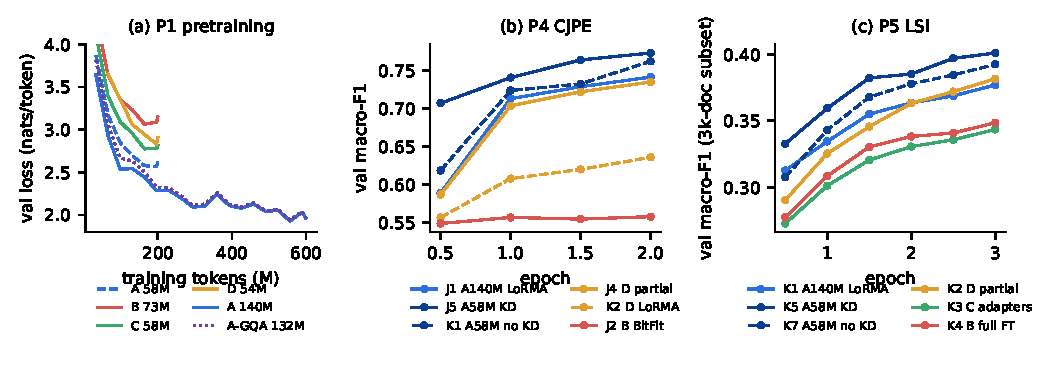
\includegraphics[width=\linewidth]{figures/fig_curves.pdf}
\caption{(a) Phase-1 validation loss vs.\ tokens (B and C losses are on continuation tokens only). (b) CJPE and (c) LSI
validation macro-F1 per half epoch.}
\label{fig:curves}
\end{figure}

Figure~\ref{fig:curves} shows that Phase-1 validation loss was still falling at 600M tokens with a small train--val
gap (2.00 vs.\ 1.96). In CJPE and LSI the KD student leads its no-teacher twin from the first evaluation, most of all
early (0.707 vs.\ 0.618 after half an epoch in CJPE), so the soft labels mainly speed up learning; BitFit stays at
chance-level loss. Across phases (Figure~\ref{fig:cross}a), the decoder-only family is first or within 4\% of first
everywhere and the encoder-decoder is last in NER, RR, CJPE and summarization. I explain this by the quality of the
pretrained representation, which follows learning signal per token and the match between pretraining and use: A
learns from every position and is fine-tuned in its pretraining attention mode, whereas B's decoder only saw
256-token continuations. The effect of technique depended on data size: LoRMA beat full fine-tuning of the same
backbone on data-poor NER (0.509 vs.\ 0.479) and RR (0.450 vs.\ 0.415), acting as a regulariser, while with 31--42k
training documents (CJPE, LSI) fully fine-tuned 58M models overtook it. Distillation (Figure~\ref{fig:cross}b) let
the student beat its teacher in CJPE (+3.7\%) and LSI (+5.5\%) at 39--43\% of the training memory and about 60\% of
the inference time; the no-teacher controls attribute half of this to distillation and half to fully fine-tuning the
smaller model. The overall winner is the decoder-only family: LoRMA on the 140M model where data are scarce or the task
is generative, and a distilled 58M student where data are plentiful.

\begin{figure}[t]
\centering
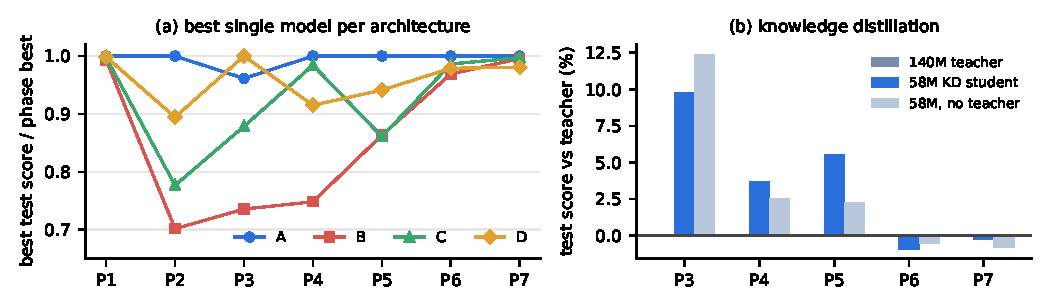
\includegraphics[width=\linewidth]{figures/fig_cross.pdf}
\caption{(a) Best single Codabench score per architecture relative to the phase's best. (b) KD student and
no-teacher student relative to the 140M teacher (P3 teacher: full FT; P6: sequence-level KD).}
\label{fig:cross}
\end{figure}

% ============================================================
\section{Error Analysis and Discussion}
% ============================================================
\subsection{Phase-wise failure modes}
\textbf{Phase~1} continuations sometimes loop (``** ** **'', chains of statute numbers); four of 1{,}000 outputs stayed
short even with 512 tokens. \textbf{Phase~2}: \textsc{auth} causes half of the best model's 666 validation false
positives, because generic words (``Government'', ``Board'') are tagged everywhere but annotated only in some contexts.
Boundary errors follow (196 spans too short, such as ``Th''+``ukral''; 121 too long, such as ``Delhi High Court'' vs.\
gold ``High Court''), while wrong labels are rare (89) and are role confusions (\textsc{resp}$\rightarrow$\textsc{app}
22). \textsc{app}/\textsc{resp} stay hardest (validation F1 at most 0.29): the ensemble misses 97 of 165 mentions,
because a party's role is stated only in the header. \textbf{Phase~3} models fall back on the majority role:
RatioOfTheDecision is predicted 710 times for 403 gold dev sentences, RulingByLowerCourt (26 of 102), None (13 of 33)
and Issue (6 of 15) are under-predicted, and the main confusions need document-level reading (petitioner vs.\
respondent arguments 103, facts vs.\ ratio 83). \textbf{Phase~4}: the predicted positive rate of one run swung from 0.34
to 0.64 between evaluations before threshold tuning, and LoRMA at learning rate $5\times10^{-4}$ collapsed to a constant
predictor. \textbf{Phase~5}: per-statute F1 rises from 0.31 (rarest fifth) to 0.54 (most frequent), misses of frequent
statutes are confusions inside one cluster (5, 34, 39, 43, 97), and documents with one gold statute receive 3.2
predictions while those with seven or more receive 6.9 for 8.7 gold. \textbf{Phase~6}: weak models invent facts (79\% of
the numbers in B's summaries are absent from the source vs.\ 31\% for the best model), the best model still shows local
loops and garbled amounts, and references above $\approx$800 words lose 0.12 ROUGE-1 to the 512-token cap.
\textbf{Phase~7}: the neural score mainly re-weights BM25 (best $w$ 0.1--0.2), lifting recall in the top 20 from 0.58 to
0.61; relevance lives in shared quoted passages, which a pooled representation captures poorly.

\subsection{What the metrics do not measure}
BERTScore rated every fluent legal text highly: halving Phase-1 perplexity moved it by 0.004, and the Phase-6 spread is
0.016 against 0.098 in ROUGE-1. Neither metric checks whether a summary states the right holding or invents an amount;
my weakest summarizer is the most ``abstractive'' because it hallucinates. Strict span-F1 counts ``Delhi High Court''
for ``High Court'' as two errors, and micro-F1@7 penalises a perfect ranker on queries with more than seven relevant
cases. For a firm, a leaderboard gain is therefore not evidence of legal correctness: summaries need a factuality check
of numbers and holdings, and NER output a partial-match score and human review.

\subsection{Limitations and what you would do next}
My largest model saw 600M of 4.5B tokens with validation loss still falling, and every downstream task was limited
by the 1{,}024-token context, so the next experiment is continued pretraining of A at 2{,}048--4{,}096 tokens, then
re-running LoRMA for CJPE and PCR. Architecture and technique are partly confounded; a grid of LoRMA and full
fine-tuning on all four backbones for CJPE would separate them. Small NER, RR and PCR test sets need repeated seeds and
confidence intervals. I had no human legal evaluation and did not test pipelining phases, so error propagation is
unknown. Further concrete steps are numeral-copy constraints for summaries, a cross-encoder re-ranker over the fused
top 50 in PCR, and co-occurrence-aware thresholds for rare statutes.

\subsection{Surprising findings}
First, a 58M student beat its 140M teacher on the CJPE (0.7706 vs.\ 0.7431) and LSI (0.3978 vs.\ 0.3770) test sets,
with half the gain coming from the teacher's soft labels. Second, LoRMA with 1.4\% trainable parameters beat full
fine-tuning in NER and RR rather than merely approaching it. Third, sequence-level distillation hurt summarization
(0.8346 vs.\ 0.8379): the teacher's summaries are shorter and 31\% of their numbers are unsupported, and the student
inherited both. Soft labels transmit a teacher's uncertainty; hard sequences transmit its mistakes.

% ============================================================
\section{Conclusion}
% ============================================================
I delivered a confidential, on-premises legal NLP stack: four from-scratch legal LMs and 72 validated submissions
over seven phases, from one laptop GPU and my own adaptation code. Three choices moved the metrics: a decoder-only
foundation trained on every token, which transferred best everywhere; LoRMA, which adapted the 140M model cheaply and
regularised it on small data; and soft-label distillation into a 58M student at about 40\% of the memory. Long-context
efficiency, header context, retraining on dev data, logit adjustment~\cite{menon2021logit}, salience-based input
selection and sequence-level distillation did not help. The main lesson is that under a parameter cap and a closed data
source, the quality of the pretrained representation and an honest, large enough validation set matter more than any
downstream trick. A skeptical partner should still not trust my summaries' numbers, my NER party roles, or score
differences below about 0.03 on the small test sets.

% ============================================================
\section*{LLM Usage Declaration}
% ============================================================
Completing this section is mandatory. Inconsistent answers relative to the code and the prose will be treated as an integrity issue.
\medskip

\noindent
\textbf{Q1.} Which Large Language Model(s), if any, did you use while completing the competition or writing this report? Give model name and vendor (e.g., none / ChatGPT-4.x / Gemini~x / Claude~x / Grok / Copilot / other). \\[0.6em]
Answer: Claude Opus 5.5 (Anthropic)
\medskip

\noindent
\textbf{Q2.} For each row, mark Yes or No and state the purpose in one short phrase. ``Yes'' is acceptable only for the uses permitted by the capstone document.
\begin{table}[H]
\centering
\begin{tabular}{>{\raggedright\arraybackslash}p{4.6cm}|c|>{\raggedright\arraybackslash}p{7.2cm}}
\toprule
Part & Used LLM? & Purpose of using the LLM \\
\midrule
Understanding concepts / papers & Yes & Explaining LoRMA, the phase tasks and related methods \\
Ideation / brainstorming at a high level & Yes & Experiment plans for each phase \\
Debugging small ancillary snippets & Yes & Windows/GPU issues, resume and format bugs \\
Plotting / visualization code & Yes & Analysis figures and the figures in this report \\
Grammar / writing style of the report & Yes & Wording of this report \\
Report structure / section wording & Yes & Drafting this report from the phase logs \\
Designing the model architecture & Yes & Code for the four Phase-1 architectures, GQA and KV cache \\
Hyperparameter search / tuning & Yes & Suggested settings and learning-rate pilots \\
Analysis of results / conclusions & Yes & Observations in the phase logs, error analyses, report draft \\
Writing the core training / inference code & Yes & All \texttt{src/} code of Phases~2--7 \\
Other (specify) & Yes & Data analysis scripts; running training queues; GitHub README files \\
\bottomrule
\end{tabular}
\end{table}
\medskip

\noindent
\textbf{Q3.} Did you refer to sources other than lecture slides and an LLM?
If yes, list them (papers, blogs, GitHub repositories, textbooks, official starter notebook, evaluation scripts). These must also appear in the bibliography when they influenced the method. \\[0.4em]
Answer: Yes. The papers in the bibliography, in particular IL-TUR~\cite{joshi2024iltur}, LoRMA~\cite{bihany2025lorma},
LoRA~\cite{hu2022lora}, knowledge distillation~\cite{hinton2015distilling,kim2016seqkd}, MobileLLM~\cite{liu2024mobilellm}
and the other adaptation and retrieval methods cited above; the official dataset card; and the capstone document.
\medskip

\noindent
\textbf{Q4.} Apart from any permitted LLM use, what was \emph{your} contribution? In 8--12 sentences describe your own understanding, architecture decisions, implementation, experiments, and analysis. Name at least two things you tried that failed and what you concluded from them.
\medskip

\noindent
Most of my own effort went into the Phase-1 foundation model, because every later phase depends on it. After the
decoder-only model won the four-way comparison at an equal 200M-token budget, I tried adjusting the total model size
to make the best use of my compute: 58M parameters on 200M tokens, then 75M on 450M tokens, and finally 140M on 600M
tokens. This lowered validation loss from 2.571 to 1.928, and the 140M model became the backbone for every later phase.
One scaling attempt failed instructively: asking for 40\% Acts in a 500M-token corpus exhausted the Acts source, which
holds only about 150M tokens, so the corpus came out at 450M tokens with a skewed mix. I concluded that the data
budget, not only the parameter count, limits a from-scratch model, and changed the data builder to pass a source's
unfilled share to the others. Halving perplexity improved BERTScore by only 0.004, which taught me not to judge the
model by BERTScore alone. When I noticed that generating the 1{,}000 test continuations took about two hours, I
decided to add grouped-query attention together with a KV cache (implemented with the LLM assistance declared above),
which shrinks the stored keys and values and cut generation to minutes with identical fp32 outputs. I then tried a
MobileLLM-style deep-thin shape (23 layers, $d$576) with GQA, expecting it to beat the wide model at equal size, but it
only tied (0.8314 vs.\ 0.8321) and trained 19\% slower, so I kept the 12-layer model and concluded that shape is not
the main lever at this scale. Downstream, sequence-level distillation in Phase~6 also failed (0.8346 vs.\ 0.8379
without a teacher) because the student copied the teacher's shorter, partly hallucinated summaries, which showed me
that hard targets pass on a teacher's mistakes while soft labels pass on its uncertainty.
\medskip

\vspace{1.4cm}
\bibliographystyle{ieeetr}
\bibliography{references}
\end{document}
